
\section{Auswertung}
\subsection{Bestimmung der Gegenspannung}
Zur Bestimmung der Gegenspannung $\su{U_G}$ der einzelnen Spektrallinien wird die Wurzel des Photostroms $\su{\sqrt{I}}$
gegen die Brems- bzw. Beschleunigungsspanunng $\su{U}$ aufgetragen. Dafür werden fünf unterschiedliche Wellenlängen ausgewählt.
Die Messergebnisse für die unterschiedlichen Farben sind aus Tabelle \ref{tab:1} zu entnehmen.
\begin{table}
\centering
\label{tab:1}
\begin{tabular}{S S S S S S}
\toprule
{$U\,/\,V$} & {$I_{\text{orange}}$\,/\,$\si{\nano\ampere}$} & {$I_{\text{grün}}$\,/\,$\si{\nano\ampere}$} & {$I_{\text{blaugrün}}$\,/\,$\si{\nano\ampere}$}\
& {$I_{\text{lila}}$\,/\,$\si{\nano\ampere}$} & {$I_{\text{dunkellila}}$\,/\,$\si{\nano\ampere}$}\\
\midrule
-0,4 & 0,030 & 0,165 & 0,026 & 1,05 & 0,79 \\
-0,2 & 0,155 & 0,450 & 0,048 & 1,40 & 0,90 \\
-0,1 & 0,235 & 0,600 & 0,056 & 1,60 & 1,00 \\
0,1 & 0,340 & 0,800 & 0,072 & 2,00 & 1,25 \\
0,2 & 0,400 & 0,900 & 0,089 & 2,20 & 1,30 \\
0,4 & 0,480 & 1,050 & 0,092 & 2,40 & 1,50 \\
0,6 & 0,560 & 1,200 & 0,105 & 2,80 & 1,75 \\
0,8 & 0,620 & 1,350 & 0,115 & 3,00 & 1,90 \\
1,0 & 0,680 & 1,500 & 0,125 & 3,40 & 2,10 \\
1,2 & 0,740 & 1,600 & 0,135 & 3,60 & 2,25 \\
\bottomrule
\end{tabular}
\caption{Aufgenomme Spannungen und Stromstärken}
\end{table}
\newline
Für die Berechnung der Gegenspannungen sind allerdings nur die Werte mit einem negativen Vorzeichen
relavant, da nur diese bei einer anliegenden Bremsspanunng aufgenommen wurden.
\newline
Die daraus resultierenden Diagramme sind in den Abbildungen \ref{fig:o} bis \ref{fig:dl} zu sehen.
\begin{figure}
  \centering
  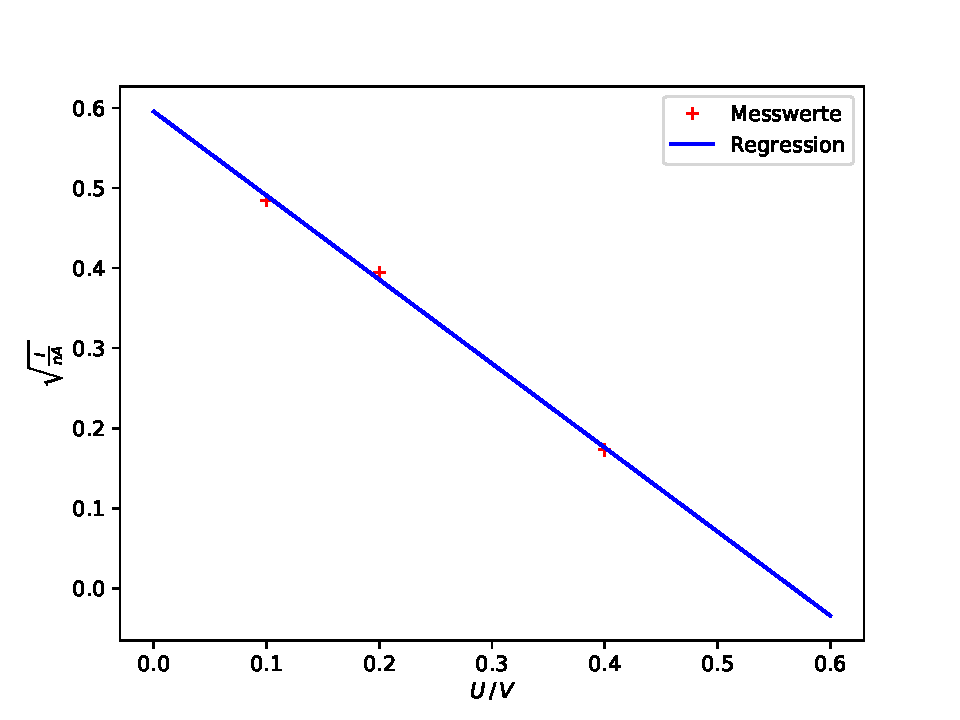
\includegraphics[scale=0.7]{orange.pdf}
  \caption{Gemessene Stromstärke in Abhängigkeit der angelegten Spannung für die orangene Spektralfarbe}
  \label{fig:o}
\end{figure}
\begin{figure}
  \centering
  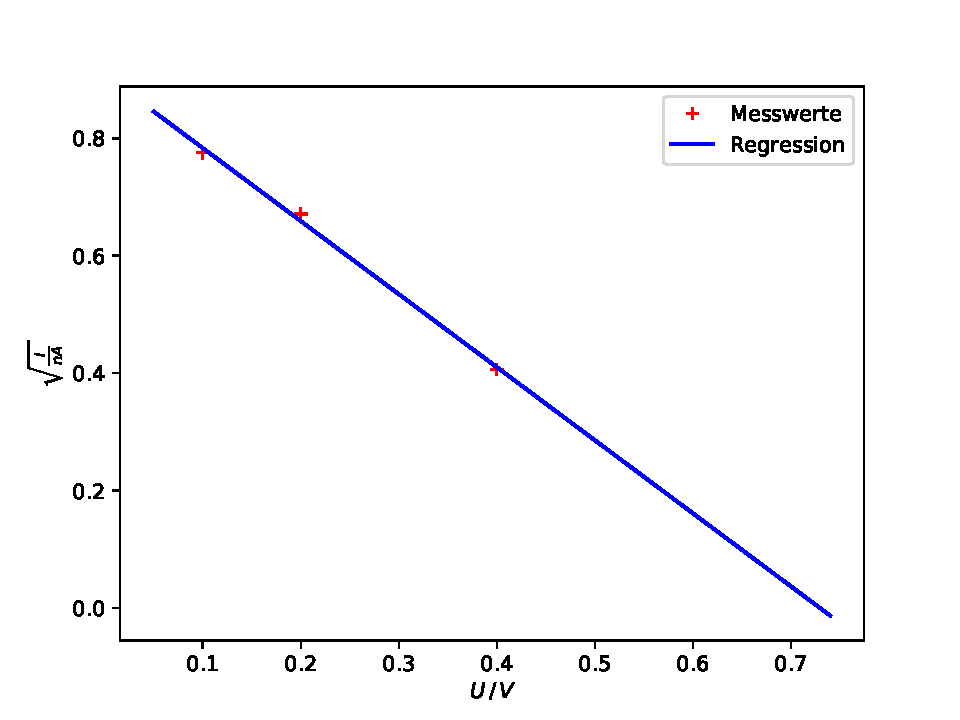
\includegraphics[scale=0.7]{grün.pdf}
  \caption{Gemessene Stromstärke in Abhängigkeit der angelegten Spannung für die grüne Spektralfarbe ($\lambda=546$\,$\si{\nano\meter}$)}
  \label{fig:g}
\end{figure}
\begin{figure}
  \centering
  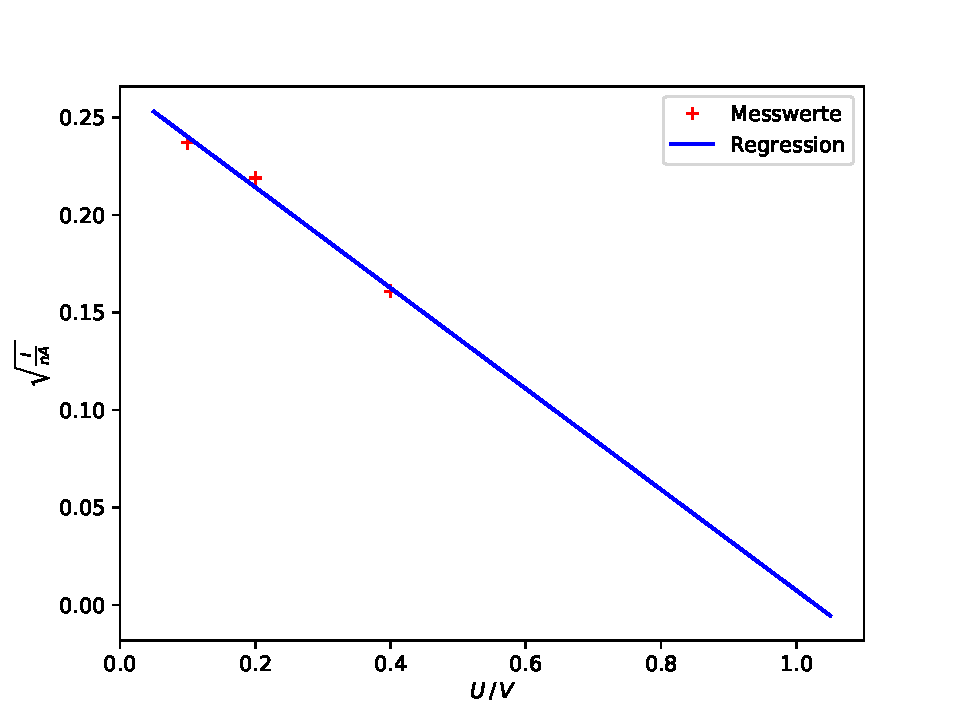
\includegraphics[scale=0.7]{blaugrün.pdf}
  \caption{Gemessene Stromstärke in Abhängigkeit der angelegten Spannung für die blaugrüne Spektralfarbe ($\lambda=492$\,$\si{\nano\meter}$)}
  \label{fig:bg}
\end{figure}
\begin{figure}
  \centering
  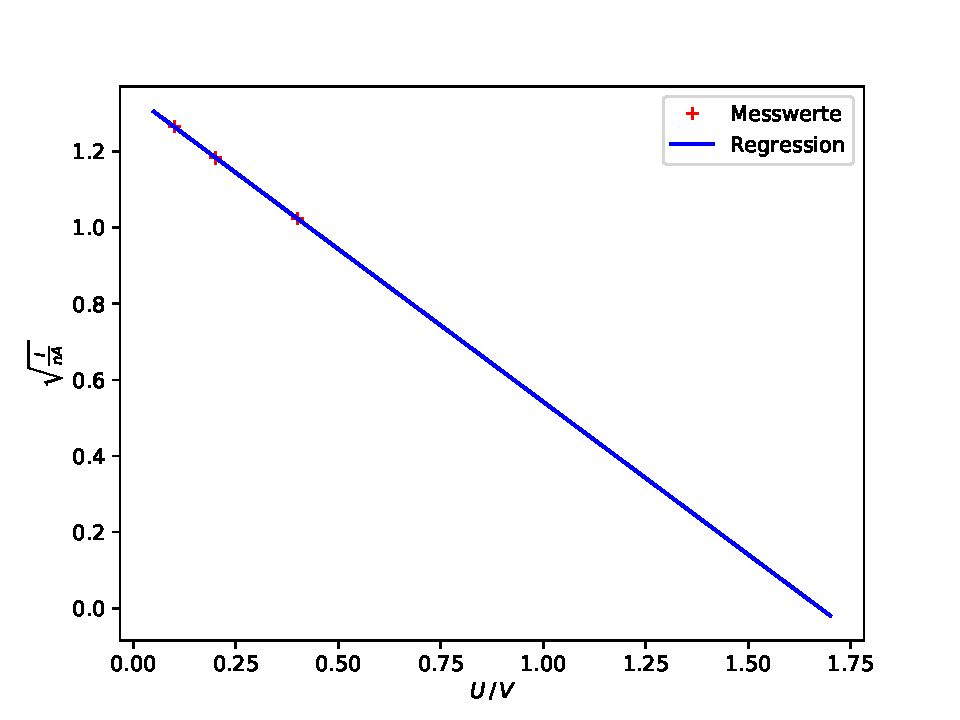
\includegraphics[scale=0.7]{lila.pdf}
  \caption{Gemessene Stromstärke in Abhängigkeit der angelegten Spannung für die lila Spektralfarbe ($\lambda=447$\,$\si{\nano\meter}$)}
  \label{fig:l}
\end{figure}
\begin{figure}
  \centering
  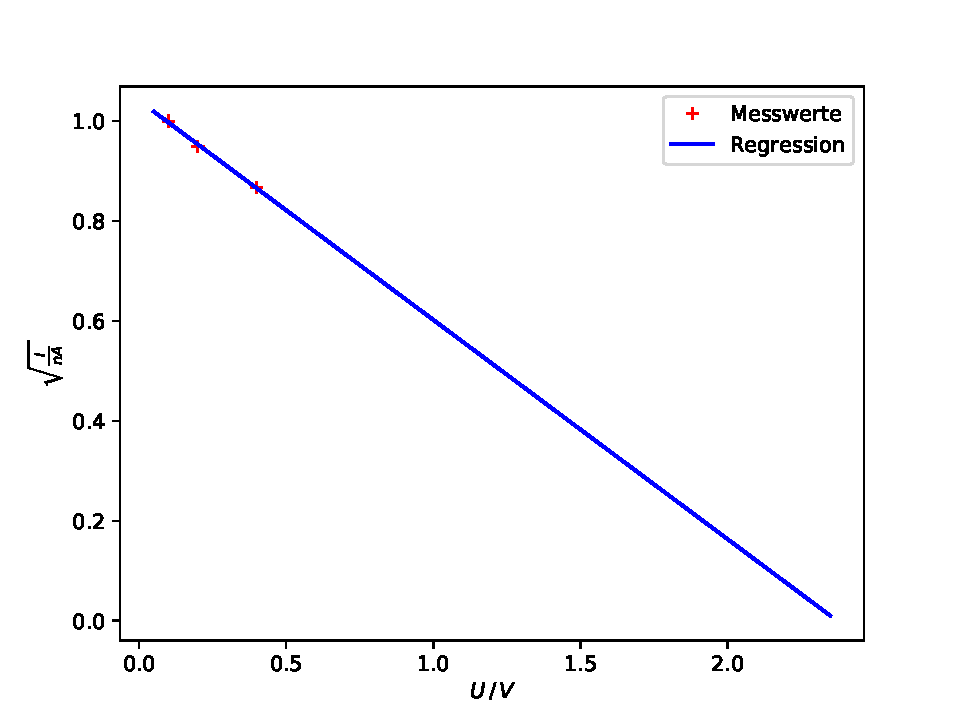
\includegraphics[scale=0.7]{dunkellila.pdf}
  \caption{Gemessene Stromstärke in Abhängigkeit der angelegten Spannung für die lila Spektralfarbe ($\lambda=438$\,$\si{\nano\meter}$)}
  \label{fig:dl}
\end{figure}
\newpage
Durch die linearen Regressionen der Form
\begin{align}
  I(U) &= a\cdot U + b
\end{align}
für die einzelnen Spektralfarben ergeben sich die Parameterwerte a, b und die
daraus resultierende Gegenspannung. Dabei ist diese genau der Schnittpunkt mit der
x-Achse. Über den Zusammenhang
\begin{align}
 U_{G} &= \frac{b}{a}
\end{align}
wird die Gegenspannung berrechnet.
\newline
Die Parameterwerte a, b und die Gegenspannungen sind in Tabelle \ref{tab:2} dargstellt.
\begin{table}
\centering
\caption{Paramaterwerte und berechnete Gegensspannung für die Spektralfarben}
\label{tab:2}
\begin{tabular}{S S S S}
\toprule
{$\lambda$\,/\,$\si{\nano\meter}$} & {$a$\,/\,$\si{\nano\ampere}$} & {$b$\,/\,$\si{\nano\ampere}$} & {$U_{G}$\,/\,V}\\
\midrule
587 & 1,050\pm0,050 & 0,5950\pm0,0130 & 0,5667\pm0,0297 \\
546 & 1,240\pm0,070 & 0,9070\pm0,0190 & 0,7314\pm0,1587 \\
492 & 0,259\pm0,027 & 0,2660\pm0,0070 & 1,0270\pm0,1104 \\
447 & 0,802\pm0,006 & 1,3445\pm0,0016 & 1,6764\pm0,0127 \\
438 & 0,439\pm0,025 & 1,0410\pm0,0070 & 2,3710\pm0,1340\\
\bottomrule
\end{tabular}
\end{table}
\newline
Der Fehler der Gegenspannung lässt sich mit der Gauß'schen Fehlerfortpflanzung
\begin{equation}
\Delta U_{G} = \sqrt{\frac{b^2}{a^4} (\Delta a)^2 + \frac{1}{a^2} (\Delta b)^2}
\label{eqn:Gauß}
\end{equation}
\newline
berechnen.
\subsection{Bestimmung des Quotienenten $\frac{h}{e_0}$ und der Austrittsarbeit}
Um die Austrittsarbeit $A_k$ und das Verhältnis $\frac{h}{e_0}$ zu bestimmen, wird zuerst
die Frequenzen $\nu$ der Spektralfarben bestimmt. Diese berechnen sich durch
\begin{align}
  \nu &= \frac{c}{\lambda}.
\end{align}
Dabei ist c die Lichtgeschwindigkeit und $\lambda$ die Wellenlänge der jeweiligen Spektralfarbe.
\newline
In Tabelle \ref{tab:f} sind die berechneten Frequenzen zu sehen und in Abbildung \ref{fig:vl}
die Gegenspannungen der unterschiedlichen Lichtfrequenzen.
\begin{table}
\centering
\caption{Berechnete Frequenzen}
\label{tab:f}
\begin{tabular}{S S S}
\toprule
{$\lambda$\,/\,$\si{\nano\meter}$} & {$\nu$\,/\,$\num{e14}$\,Hz} & {$U_{G}$\,/\,V}\\
\midrule
587 & 5,11 & 0,5667 \\
546 & 5,49 & 0,7314 \\
492 & 6,10 & 1,0270 \\
447 & 6,71 & 1,6764 \\
438 & 6,85 & 2,3710 \\
\bottomrule
\end{tabular}
\end{table}
\begin{figure}
  \centering
  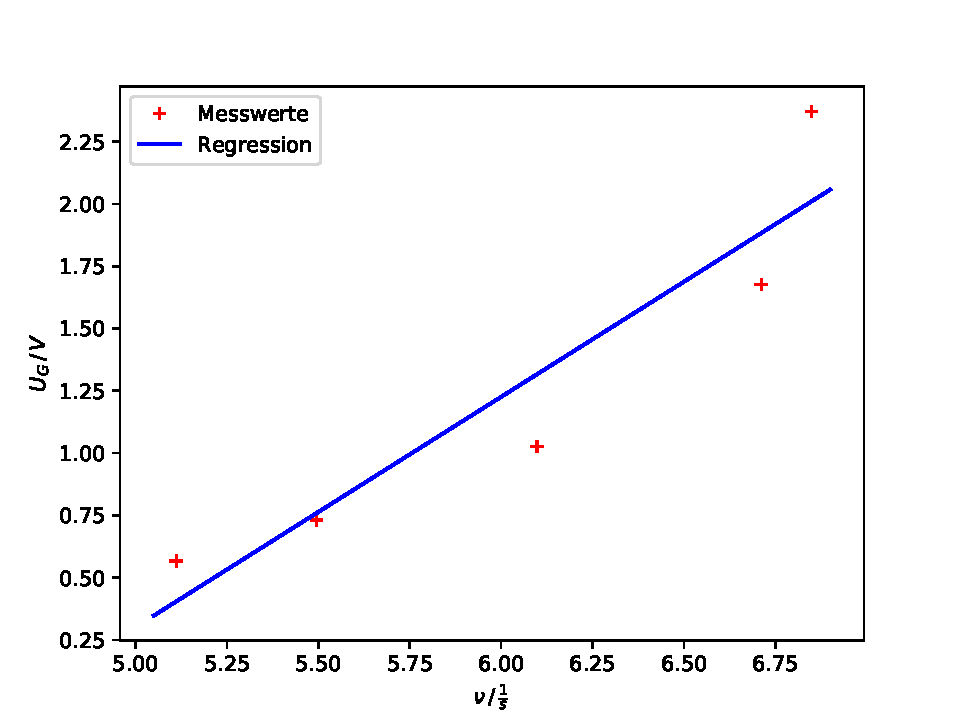
\includegraphics[scale=0.6]{frequenz.pdf}
  \caption{Gegenspannung der verschiedenen Lichtfrequenzen}
  \label{fig:vl}
\end{figure}
\newpage
Durch die lineare Ausgleichgerade der Form $U_G(\nu)=a\nu +b$ ergeben sich für die beiden
Parameter a und b folgende Werte
\begin{align*}
  a &= (6,8\pm1,1) \cdot \num{e-15}\,Vs\\
  b &= -(3,0\pm0,6) \,V
\end{align*}
Hierbei wurde die Frequenz für die dunkellilane Spektralfarbe $\lambda$ = 438\,nm aus der
linearen Regression herausgenommen. Bei dieser ist der berechnete Wert für die
Ausgangsspannung $\su{U_G}$ sehr groß, was zu einer größeren Steigung der Geraden führt
und somit zu einer größeren prozentualen Abweichung.
\newline
Die Steigung der Geranden entspricht dem Quotienten des planckschen Wirkumsquantums $\su{h}$ und der
Elementraladung $\su{e_0}$. Daraus ergibt sich der Zusammenhang
\begin{align*}
  a &= \frac{h}{e_0} = (6,8\pm1,1) \cdot \num{e-15}\,Vs.
\end{align*}
Die Austrittsarbeit beträgt dann
\begin{align*}
  A_k &= -b = (3,0\pm0,6) \,eV.
\end{align*}
\newpage
\subsection{Messung für die gelbe Spektralfarbe $\lambda$=578\,nm}
Im letzten Teil des Versuchs wird für gelbes Licht der Wellenlänge $\lambda$=578\,nm
die Spannung im Verhältnis zum Photostrom gemessen. Die Messwerte sind in Tabelle \ref{tab:Messungb}
zu sehen.
\begin{table}
  \centering
  \caption{Messung für die gelbe Spektralfarbe ($\lambda$= 578\,nm)}
  \label{tab:Messungb}
  \begin{tabular}{c c}
    \toprule {$U\,/\,V$} & {$I$\,/\,$\si{\nano\ampere}$}\\
    \midrule
-0,5 & 0,008 \\
-0,4 & 0,034 \\
-0,3 & 0,085 \\
-0,2 & 0,185 \\
-0,1 & 0,265 \\
0,1 & 0,380 \\
0,5 & 0,560 \\
1,0 & 0,760 \\
2,0 & 1,250 \\
3,0 & 1,750 \\
4,0 & 2,050 \\
5,0 & 2,200 \\
6,0 & 2,350 \\
7,0 & 2,500 \\
8,0 & 2,700 \\
9,0 & 2,800 \\
10,0 & 3,000 \\
11,0 & 3,000 \\
12,0 & 3,200 \\
14,0 & 3,200 \\
16,0 & 3,400 \\
19,0 & 3,600 \\
\bottomrule
\end{tabular}
\end{table}
\begin{figure}
  \centering
  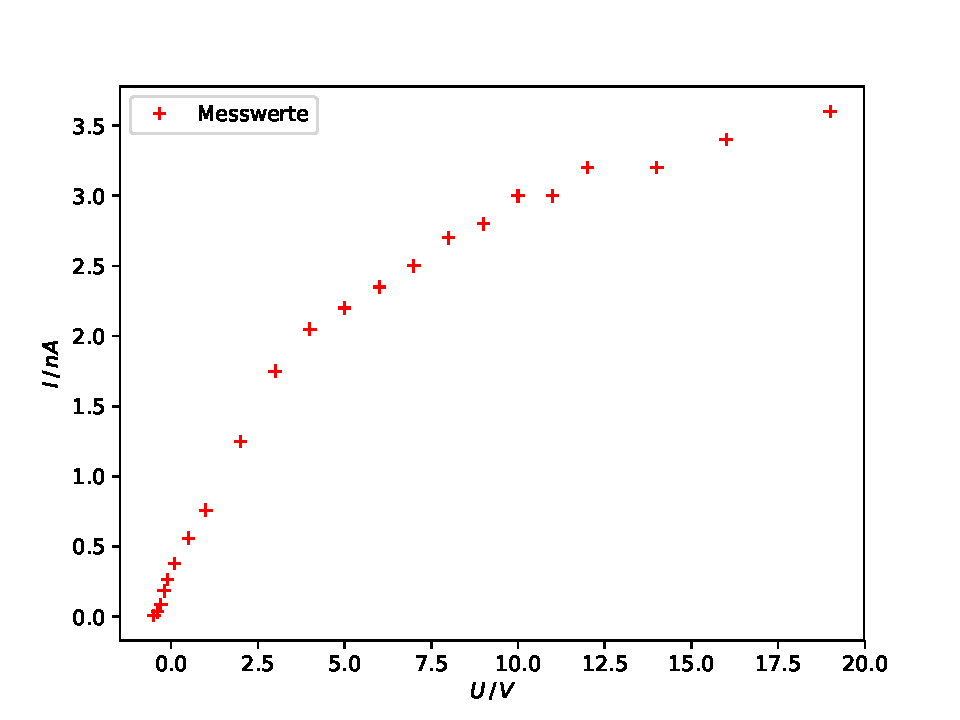
\includegraphics[scale=0.6]{gelb.pdf}
  \caption{Gemessene Stromstärke in Abhängigkeit der anglegten Spannung für die gelbe Sprektralfarbe}
  \label{fig:gelb}
\end{figure}
\newpage
In Abbildung \ref{fig:gelb} ist der Kurvenverlauf des Photostroms in Abhänigkeit der Spannnung
für $\lambda$=578\,nm zu sehen.
\newline
Auffällig am Kurvenverlauf ist die Konvergenz gegen einen bestimmten Sättigungswert für hohe
beschleunigenden Spannungen. Dieser Sättigungswert lässt sich dadurch erklären, dass nur eine
bestimmt Anzahl von Elektronen aus der Festkörperoberfläche herausgelöst werden kann. Nur von
der Lichtintensität hängt diese Elekronenanzahl ab.
\newline Das Ohmsche Gesetz beschreibt einen proportional ansteigenden Strom in Abhängigkeit der
Spannung. Da die Anzahl der Ladungsträger aber in diesem Versuch begrenzt ist, kann das Ohmsche
Gesetz hier nicht erfüllt werden.

Der Grund für das asymptotische Verhalten am Grenzwert ist die Elektronenstreuung, weshalb
einige Elektronen die Anode nicht erreichen. Um diesen Elektronenverlust zu verhindern,
müsste die Oberfläche der Anode vergrößert werden.

Beim Anlegen einer Gegenspannung fällt der Photostrom aufgrund der Fermi-Dirac-Verteilung
nicht aprupt auf 0 ab. Diese Verteilung beschreibt die Energieverteilung der Elektronen
im Festkörper, wobei ausgelöste Elektron häufige unterschiedliche Energien besitzen.

Zur Beobachtung eines negativen Photostroms muss nur die Bremsspanunng groß genug
eingestellt werden. Dies führt allerdings dazu, dass der Photostom der Kathode überlagert wird.
Von der Anode ausgehend werden Elektronen zur Kathode hin beschleunigt. Dieser negative Photostrom
erreicht durch die geringe Freisetzung ausgelöster Elektronen einen kleineren Sättigungwert.

Unter der Einstrahlung von energiearmen Licht tritt bereits der negative Strom auf.
Somit ist die Austrittsarbeit der Anode an die Austrittarbeit der Kathode festgelegt.
\section{Diskussion}
Bei der Bestimmung der Regresionsparamter traten nur kleine Fehler auf. Allerdings konnten
diese immer nur aus drei Wesswerten bestimmt werden, da alle anderen Werte bei einer Beschleunigungsspanunng
aufgenommen wurden.
\newline
Beim Auftragen der Gegenspannungen gegen die Frequenz sind schon deutlich größere
Abweichungen zu erkennen. Das Ergebnis für den Quotienten aus dem planckschen Wirkungsquantum $\su{h}$
und der Elementraladung $\su{e_0}$ ist im Vergleich zum Literaturwert nochmal aufgelistet:
\begin{align*}
  (\frac{h}{e_0})_{\su{experimentell}} &= 6,8\,eV \\
  (\frac{h}{e_0})_{\su{Literatur}} &= 1.436\,eV.
\end{align*}
\newline
Der berechnete Quotient $\frac{h}{e_0}$ weist mit einer prozentualen Abweichung von
374\,$\%$ einen großen Fehler zum Literaturwert \cite{Wert} auf. Die prozentuale Abweichung wird durch den Betrag von
\begin{equation}
  \Delta{C} = \frac{C_\su{experimentell}-C_\su{Literatur}}{C_\su{Literatur}}
\end{equation}
\newline
bestimtt.
Dieser große Fehler lässt sich vor allem auf die letzte Messung der dunkellilanen
Spektralfarbe mit $\lambda$ = 438\,nm zurückführen. Während der Messreihe hat sich dort
merklich das emittierte Licht der Lampe nicht mehr auf die Photokathode konzentriert.
Hier ist es gut möglich, dass ein Teil einer anderen Spektrallinie mitgemessen wurde.
Die gemessene Gegenspannung von $U_G$ = 2,371\,V lässt zu mindest darauf schließen, dass dies
die größte Fehlerquelle war.
\newline
Auch bei den anderen Spektralfarben lassen sich Abweichungen feststellen, die sind allerdings deutlich
geringer als die der dunkellilanen. Diese lassen sich aber durch den nicht komplett abgedunkelten
Raum und auf die Empfindlichkeit der Messgeräte zurückführen.
\newline
Die angesprochenen Fehler und besonders die geringe Anzahl an Messwerten führen zu der großen
prozentualen Abweichung, weshalb der Quotient nicht besonders aussagekräftig
erscheint.
\newline
Trotzdem lassen sich in diesem Versuch die experimentell gewonnen Ergebnise des Photoeffekts gut erkennen.
